\chapter{Metodología de detección de sismos}
\label{cap:deteccion}

Uno de los objetivos específicos de esta tesis es proveer una metodología no supervisada para detectar la ocurrencia de sismos. 
%
Con la finalidad de contribuir al estado del arte, se busca que la metodología propuesta permita detectar sismos en cualquier parte del mundo en tiempo cercano al tiempo real (entre 0 y 5 minutos) y que no dependa de procesos de clasificación supervisada de los mensajes (por lo tanto, que no tenga costos asociados al trabajo de etiquetado). 


El algoritmo utilizado para la detección de sismos es una adaptación de un enfoque no supervisado de detección de anomalías en flujos de texto presentado por Guzmán y Poblete~\cite{guzman2013line}. 
%
El algoritmo original permite detectar eventos emergentes al analizar el flujo genérico de mensajes publicados en Twitter de forma eficiente.  
%
Esta adaptación formaliza el algoritmo original para ser utilizado para monitorizar 
%señales de tiempo discretas menos genéricas que son creadas a partir del flujo de mensajes de Twitter
flujos de mensajes menos genéricos que son creados a partir del flujo de mensajes de Twitter, en este caso en particular, un flujo de mensajes relacionados con sismos.

Se escoge este método porque tiene una complejidad lineal (en relación al número de mensajes de la entrada) y porque la configuración inicial es simple, requiriendo solamente el ajuste de algunos parámetros.
%
Otras técnicas de detección de eventos requieren ajustar periódicamente los parámetros~\cite{mathioudakis2010twittermonitor,sankaranarayanan2009twitterstand} o tienen complejidad computacional mayor, como las propuestas por Zhou et al.~\cite{zhou2015unsupervised} y Zhao et al.~\cite{zhao2014unsupervised} que tienen complejidad polinomial y cuadrática respectivamente. 

%\jm{Mencioné esto aquí, no sé si es suficiente o si lo pongo además como una nota al pie de página}
El trabajo descrito en este capítulo y la correspondiente evaluación descrita en el capítulo \ref{cap:analisis}, se realizó en colaboración con Jheser Guzmán como parte de su trabajo de doctorado.


\section{Velocidad de llegada relativa}

El algoritmo original propuesto por Guzmán y Poblete se basa en comparar ventanas de tiempo consecutivas y detectar variaciones considerables entre la velocidad de llegada relativa calculada para las palabras que componen los mensajes en cada ventana de tiempo.

Para definir formalmente la velocidad de llegada relativa se considera ${\mathcal F} = \langle F_1, F_2, \dots, F_n \rangle$ un flujo de mensajes indexados por tiempo , donde  $t: {\mathcal F} \rightarrow \mathbb{R}^+$ indica el tiempo de llegada de los mensajes, $F_i \subseteq A$ es el conjunto de atributos del mensaje $F_i$ y $A$ es el conjunto de posibles atributos de los mensajes entre los que se encuentran las palabras clave, localidades, \textit{hashtags}, sentimiento inferido, entre otros.  

En el conjunto de posibles atributos en $A$ existen algunos que constituyen \emph{elementos de interés}, los cuales dependen de lo que se quiera detectar (en este caso, atributos que podrían estar relacionados con sismos) y que se denotan como $K \subseteq A$.

Además se denotan:
\begin{itemize}
	\item $w_i = \langle w^s_i, w^e_i \rangle$ como una ventana de tiempo que abarca desde el tiempo $w^s_i$ hasta el tiempo $w^e_i$.
 	\item $M_i = \{ s \in {\mathcal F}: w^s_i \le t(s) \le w^e_i \}$ como el conjunto de los mensajes de ${\mathcal F}$ dentro de la ventana de tiempo. 
	\item $\operatorname{freq}(K, M_i) = | \{ F \in M_i: K \cap F \neq \emptyset \} |$ como cantidad de mensajes dentro $M_i$ que contienen elementos de interés.
\end{itemize}

Finalmente, en el método propuesto, el flujo de datos es procesado en grupos, dividiendo los mensajes que llegan en ventanas de tiempo consecutivas de largo fijo $T$.

Considerando todo lo anterior, para una ventana de tiempo dada $w_i$ que contiene los mensajes $M_i$, se define la \emph{velocidad de llegada relativa} ($\lambda$) de elementos de interés en esta ventana como:

\begin{equation}
\label{eq:lambda}
\lambda(K, M_i) = \frac{\mathrm{freq}(K,M_i)}{T|M_i|}
\end{equation}

\section{Adaptación de la metodología de detección}

La metodología propuesta se basa en monitorear el flujo de mensajes ($\mathcal{F}$) en el tiempo, para determinar cuándo una variación positiva en la velocidad de llegada relativa ($\lambda$) de elementos de interés es significativamente más grande que otras variaciones producidas por el ruido observado en el pasado.
%
Originalmente, en el método propuesto por Guzman y Poblete, la ``explosividad'' de cada palabra es estimada en base a la magnitud del cambio de su velocidad de llegada relativa ($\lambda$) con respecto a la ventana de tiempo previa.
%
La salida es una lista de los top-\emph{k} términos ordenados en orden decreciente según el cambio de su velocidad de llegada relativa ($\lambda$).
%
Pero esto no es suficiente para el propósito de la detección de sismos. 

Para el caso de la detección de sismos los datos que conforman el flujo se seleccionan a partir de palabras clave\footnote{El proceso de recolección se detalla en la sección \ref{sec:recoleccion}.}. 
%
Esto implica que el flujo a monitorear sea un flujo sesgado, en el que hay pocas palabras muy frecuentemente usadas (menos de \emph{k} palabras) y que experimentan pequeños cambios en cada ventana de tiempo debido a fluctuaciones al azar en los datos de entrada (i.e., ruido).
%
Por lo tanto, si se reportan las top-\emph{k} palabras más ``explosivas'' podría significar tener reportes en cada ventana de tiempo.
%
Es por esto, que para reportar sismos automáticamente se necesita estimar, de forma confiable, cuándo un cambio es significativo y por lo tanto indica actividad inusual.

\begin{figure}[h]
\minipage{0.46\textwidth}
 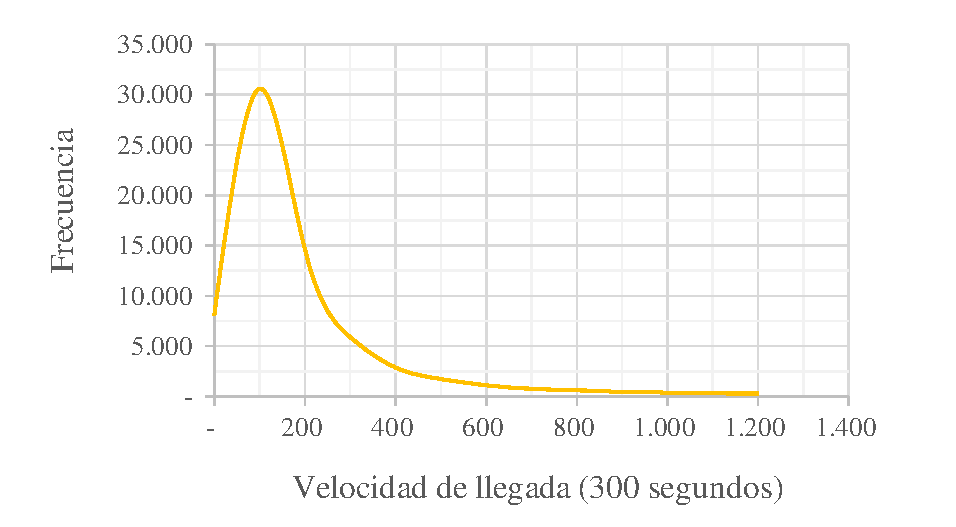
\includegraphics[trim={20 6 0 6}, clip, width=\linewidth]{imagenes/distribucion_02.pdf}
 \caption{Distribución de la frecuencia de los mensajes relacionados con sismos en ventanas de tiempo de 300 segundos.}
 \label{fig:data_distribution1}
\endminipage\hfill
\minipage{0.46\textwidth}
  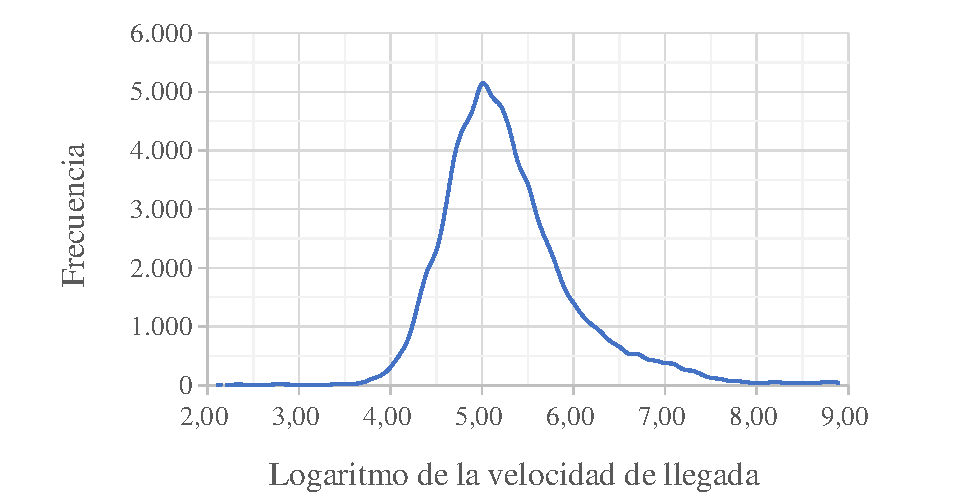
\includegraphics[trim={20 0 0 0}, clip, width=\linewidth]{imagenes/distribucion_03.pdf}
  \caption{Distribución del logaritmo de la frecuencia de los mensajes relacionados con sismos en ventanas de tiempo de 300 segundos.}
  \label{fig:data_distribution2}
\endminipage\hfill
\end{figure}


El enfoque natural para determinar si la velocidad de llegada relativa ($\lambda$) experimenta una variación significativa durante una ventana de tiempo $w_i$ es monitorizar la desviación estándar de $\lambda$ para todas las ventanas de tiempo hasta $w_{i-1}$; al igual que como se ha hecho en el trabajo previo sobre detección de eventos emergentes usando enfoques estadísticos basados en la distribución de frecuencias~\cite{kleinberg2003bursty, mathioudakis2010twittermonitor,
nguyen2013event}.
%
Esta idea asume y requiere que la velocidad de llegada relativa ($\lambda$) tenga una distribución exponencial. 
%
Sin embargo, un análisis empírico cuyo resultado se muestra en la figura ~\ref{fig:data_distribution1}, usando el conjunto de datos recolectados durante un período de 9 meses desde el 25 de Enero al 25 de Octubre del 2016, indica que esto no se cumple para el caso de la distribución de la velocidad de llegada de las palabras relacionadas con sismos.
%
Esta observación hizo necesario un análisis para identificar como adaptar el algoritmo a los propósitos descritos en esta tesis.


Entre los análisis realizados hay uno en particular que resultó útil para continuar. Se aplicó una transformación logarítmica a los datos, tal como se muestra en la figura~\ref{fig:data_distribution2}, después de lo cual los datos se asemejan a una distribución {\em log-normal}.
%
Por lo tanto, en vez de monitorizar los cambios en la velocidad relativa de llegada ($\lambda$), se modeló la distribución como si fuera {\em log-normal} y se monitorizan los cambios en el logaritmo de la función. La función transformada se define como:

\begin{equation}
\label{eq:log_lambda}
\tilde{\lambda}(K, M_i) = \frac{\ln\left(\mathrm{freq}(K,M_i)\right)}{T |M_i|}
\end{equation}

Usando la función transformada $\tilde{\lambda}(K, M_i)$ se calculó su {\em z}-score\footnote{El z-score (standard score) indica a cuántas desviaciones estándar se encuentra un elemento de la media}. Este valor es monitorizado para identificar las variaciones significativas.  

\newcommand{\zscore}{\ensuremath{z\textnormal{-}\mathrm{score}}}
\begin{equation}
\label{eq:zscore}
\zscore(K, M_i) = \frac{\tilde{\lambda}(K, M_i)-\mu_i}{\sigma_i}
\end{equation}

\noindent donde $\mu_i$ y $\sigma_i$ son, respectivamente, el promedio y la desviación estándar de los valores observados de $\tilde\lambda$ durante las ventanas de tiempo $w_1, w_2, \dots, w_{i-1}$.

El método propuesto monitoriza la señal discreta formada por los valores del {\em z}-score calculado para cada ventana de tiempo y cataloga como una detección de sismo cada uno de los instantes en donde $\zscore(K, M_i)\ge\theta$, donde $theta$ es un umbral definido experimentalmente.
%
En el capítulo~\ref{cap:analisis} se describen los experimentos realizados para determinar los parámetros iniciales y el valor del umbral para $\theta$. 
